\documentclass[12pt, onecolumn]{article}

% Set the page margins to 1 inch on all sides
\usepackage[margin=1in]{geometry}

% Improved font encoding
\usepackage[T1]{fontenc}
\usepackage{lmodern}

% Packages for title and section formatting
\usepackage{titlesec}
\usepackage{titling}

% Packages for math, images, tables, code listings, hyperlinks, and custom spacing
\usepackage{amsmath, amssymb, amsfonts}
\usepackage{graphicx}
\usepackage{xcolor}
\usepackage{booktabs}
\usepackage{graphicx} % for \resizebox
\usepackage{pdflscape} % for landscape tables
\usepackage{minted}
\usepackage{hyperref}
\usepackage{fancyhdr}
\usepackage{setspace}

% For code listings
\usemintedstyle{manni}
\setminted{
  frame=lines,
  framesep=2mm,
  baselinestretch=1.2,
  bgcolor=lightgray,
  fontsize=\footnotesize,
}
% Define a custom color for the background
\definecolor{LightGreen}{rgb}{0.95, 1, 0.95} % RGB values for a light green color

% Set up minted environment for code highlighting with the new background color
\setminted[matlab]{
  frame=lines,
  framesep=2mm,
  baselinestretch=1,
  bgcolor=LightGreen,
  fontsize=\footnotesize,
}
% Hyperlink setup
\hypersetup{
    colorlinks=true,
    linkcolor=blue,
    filecolor=magenta,
    urlcolor=cyan,
}
\urlstyle{same}

% Header and footer setup
\pagestyle{fancy}
\fancyhf{}
\rhead{EE6227 Genetic algorithms and machine learning}
\lhead{Experiment Report}
\rfoot{Page \thepage}

% Title, author, and date setup
\title{\vspace{-2em}Machine Learning Assignment 1\&2 - Classification}
\author{\small Deng Haoyuan G2303928A \\
\small School of Electrical and Electronic Engineering \\
\small Nanyang Technological University \\
\small E230112@e.ntu.edu.sg}
\date{\vspace{-2em}} % Remove space after date

% Adjusting spacing for sections and subsections
\titlespacing*{\section}{0pt}{1.25ex plus 1ex minus .2ex}{0.75ex plus .2ex}
\titlespacing*{\subsection}{0pt}{1.0ex plus 1ex minus .2ex}{0.5ex plus .2ex}

\begin{document}
\maketitle
\thispagestyle{fancy} % Apply fancy header and footer to first page
\setstretch{0.5}
\begin{singlespace}
\begin{abstract}
This comprehensive report delineates the approaches and outcomes of two sequential assignments within the realm of machine learning, specifically focusing on pattern classification. In Assignment 1, the study is anchored around the empirical training and performance evaluation of three classifiers: \textbf{the Bayes decision rule, Gaussian Naïve Bayes, and Linear Discriminant Analysis}. These classifiers were systematically trained using a designated dataset partitioned into training and test segments. The core objective was to develop models capable of accurately predicting the class labels of 26 test data samples. Special attention was given to the \textbf{Gaussian Naïve Bayes classifier}, leveraging its assumption of normally distributed features to model the probabilities. Assignment 2 pivots to preliminary data analysis, probing for and addressing missing values and outliers within the training dataset. It encapsulates the strategic methodology employed for data cleansing and the rationale behind such methods. Additionally, the task includes the construction and utilization of a \textbf{binary classification tree} to predict the class labels of 30 unlabeled test data samples. The synthesis of these assignments illustrates the critical role of effective data handling and algorithmic selection in enhancing the predictive performance of machine learning models.
\end{abstract}
\end{singlespace}
\setstretch{1.15}

\section{Assignment 1}
\subsection{Analysis of Data samples}
Initial data analysis was conducted to understand the dataset's distribution for selecting an appropriate Naïve Bayes classifier. The `data\_train. mat`, `label\_train.mat`, and `data\_test.mat` samples were analyzed, focusing on the class categories, quantity of data points, dimensionality, and the number of test samples. and the number of test samples. The Gaussian Naïve Bayesian classifier was applied to continuous data, while the Bernoulli and polynomial classifiers were applied to binary and discrete data, respectively. The histogram in Figure \ref{fig:histogram} shows the average distribution of the categories in the training set, and it can be seen that there are a total of two categories, each with 210 sample points respectively; Table \ref{tab:data_dimensions} shows the dimensionality of the data in the three files. Since the dimension of the sample points is 5, it is not convenient to visualize their distribution, \textbf{so we first use PCA to reduce it to 2 dimensions to show its distribution on the first two main feature vectors}, and Fig. \ref{fig:pca_scatter} shows the scatterplot after the PCA reduction to show the dispersion characteristics of the data.

% Include your MATLAB code within the minted environment for syntax highlighting
\begin{minted}{matlab}
% Load the datasets
load('data_train.mat'); % load the training data
load('label_train.mat'); % load the labels for the training data
load('data_test.mat'); % load the test data

% Display variable information
whos;
% Observe the first few samples
% disp(data_train((1:5),:));
% disp(label_train((1:5),:));

% Output the type and amount of data
class_label = unique(label_train);
class_number = histc(label_train, class_label);

% Bar plot code ...
for i = 1:length(class_label)
    bar(class_label(i), class_number(i), 'FaceColor', colors(i,:), 'EdgeColor', 
       'none', 'LineWidth', 1.5);
    hold on; 
end
for i = 1:length(class_label)
    %fprintf('numbers of class %d : %d\n',class_label(i),class_number(i));
    text(class_label(i), class_number(i) + max(class_number), sprintf('%d', 
    class_number(i)), ...
         'HorizontalAlignment', 'center', ...
         'VerticalAlignment', 'bottom' ,'FontSize',12,'Color',[0 0 0]);
    hold on;
end
% PCA and scatter plot code 
[coeff, score, ~, ~, explained] = pca(data_train);
reduced = score(:,1:2);
figure;
gscatter(reduced(:,1),reduced(:,2),label_train);
\end{minted}

\begin{figure}[htbp]
\centering
\begin{minipage}[b]{0.48\linewidth}
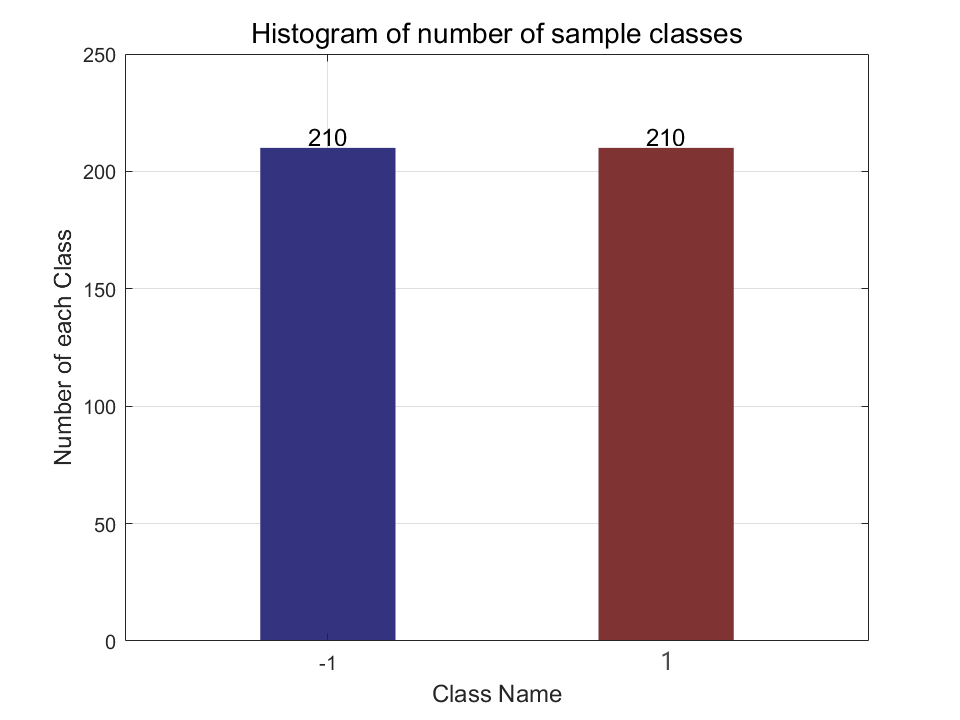
\includegraphics[width=\linewidth]{Bar.png}
\caption{Histogram of number of sample classes.}
\label{fig:histogram}
\end{minipage}
\hfill
\begin{minipage}[b]{0.48\linewidth}
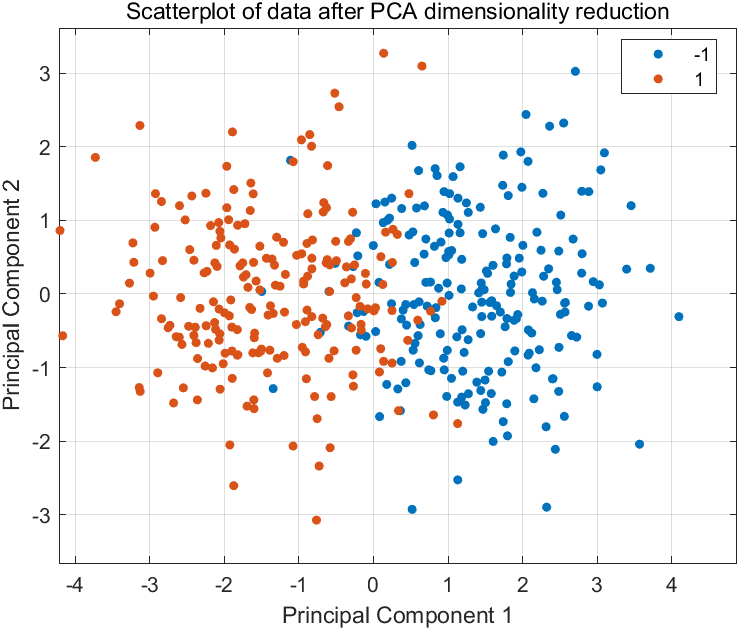
\includegraphics[width=\linewidth]{PCA降维分布1.png}
\caption{Scatterplot of data after PCA dimensionality reduction.}
\label{fig:pca_scatter}
\end{minipage}
\end{figure}

\begin{table}[htbp]
\centering
\begin{tabular}{lc}
\hline
\textbf{File Name} & \textbf{Dimensions} \\
\hline
\texttt{data\_train} & \(420 \times 5\) \\
\texttt{data\_test}  & \(26 \times 5\)  \\
\texttt{label\_train} & \(420 \times 1\) \\
\hline
\end{tabular}
\caption{Dimensions of the data files.}
\label{tab:data_dimensions}
\end{table}

% Continue with the rest of your document...
% Other sections go here

\subsection{Bayesian Decision Classifier}
Let $\mathbf{x}$ denote the feature vector, and $\{\omega_1, \omega_2, \ldots, \omega_c\}$ denote the $c$ classes (in this project, $c = 2$ and the feature dimension is 5). In Bayes decision rule, the posterior probability is used as the discriminant function:
\[
g_i(\mathbf{x}) = p(\omega_i|\mathbf{x}) = \frac{p(\mathbf{x}|\omega_j)p(\omega_j)}{p(\mathbf{x})} = p(\mathbf{x}|\omega_i)p(\omega_i) , \quad i = 1,2, \ldots, c
\]
It can be seen that since ${p(\mathbf{x})}$ is equal for both classes, the discriminant equation is ultimately determined by the class conditional probability density $p(\mathbf{x}|\omega_i)$ and the prior probability $p(\omega_j)$ . We assume that the sample data distribution obeys the Multivariate normal density function:

\[
p(\mathbf{x}|\omega) = \frac{1}{(2\pi)^{d/2}|\mathbf{\Sigma}|^{1/2}} \exp \left[ -\frac{1}{2} (\mathbf{x} - \mathbf{\mu})^T \mathbf{\Sigma}^{-1} (\mathbf{x} - \mathbf{\mu}) \right]
\]

Then, since both the mean \(\mathbf{\mu}\) and covariance \(\mathbf{\Sigma}\) of the original data are unknown, we use maximum likelihood estimation to obtain them. With a similar derivation process, the maximum-likelihood estimate of \(\mathbf{\mu}\) and \(\mathbf{\Sigma}\) are obtained as follows:
\[
\hat{\mathbf{\mu}} = \frac{1}{n} \sum_{k=1}^{n} \mathbf{x}_k
\]

\[
\hat{\mathbf{\Sigma}} = \frac{1}{n} \sum_{k=1}^{n} (\mathbf{x}_k - \hat{\mathbf{\mu}})(\mathbf{x}_k - \hat{\mathbf{\mu}})^T
\]

Along these lines, our code is as follows, which first calculates the prior probabilities of different categories, and then calculates the statistical parameters of different sample categories to estimate the overall statistical parameters of the category:
\begin{minted}{matlab}
% Calculating the priori probabilities
unique_labels = unique(label_train);
priors = zeros(length(unique_labels), 1);
for i = 1:length(unique_labels)
    priors(i) = sum(label_train == unique_labels(i)) / length(label_train);
end

% Calculate statistical parameters for each class
means = zeros(length(unique_labels), size(data_train, 2));
variances = zeros(length(unique_labels), size(data_train, 2));
for i = 1:length(unique_labels)
    class_data = data_train(label_train == unique_labels(i), :);
    means(i, :) = mean(class_data, 1);
    variances(i, :) = var(class_data, 0, 1); 
end
\end{minted}

After obtaining the statistical parameters of the two categories, the following discriminant equation is calculated to determine the category to which the sample points of the test dataset belong:
\begin{minted}{matlab}
% Applying Bayesian decision rules for classification
predicted_labels = zeros(size(data_test, 1), 1);
for i = 1:size(data_test, 1)
    posteriors = zeros(length(unique_labels), 1);
    for j = 1:length(unique_labels)
        % Calculate the conditional probability density 
        likelihood = (1 ./ sqrt(2 * pi * reshape(variances(j, :), 1, []))) .* ...
                     exp(-((data_test(i, :) - means(j, :)).^2 ./ (2 * 
                     reshape(variances(j, :), 1, []))));
        % Compute the posterior probability    
        posteriors(j) = prod(likelihood) * priors(j);
    end
    % Select the class with the maximum posterior probability
    [~, predicted_index] = max(posteriors);
    predicted_labels(i) = unique_labels(predicted_index);
    disp(['Sample ' num2str(i) ', Predicted label: ' num2str(predicted_labels(i))]);
end

disp('Predicted labels:');
disp(predicted_labels);
\end{minted}

Based on the above code, we classify the test data according to the discriminant, Table \ref{tab:mean_variance} shows the mean and eigenvectors of the two sample data point categories, and the posterior probability is calculated as the discriminant based on the likelihood ratio, and those with large values are grouped into the same category. We first counted the number of each test category that had a Bayesian decision classifier discriminant, noting that after the three classifiers section of Assignment 1, we will analyze the classification of each test sample point by the three classifiers in a uniform manner. As shown in Figure \ref{fig:prediction_results}, 15 of the test samples were categorized as category '-1' and 11 sample points were categorized as category '1'.

\begin{figure}[htbp]
  \centering
  \begin{minipage}{0.5\textwidth}
    \centering
    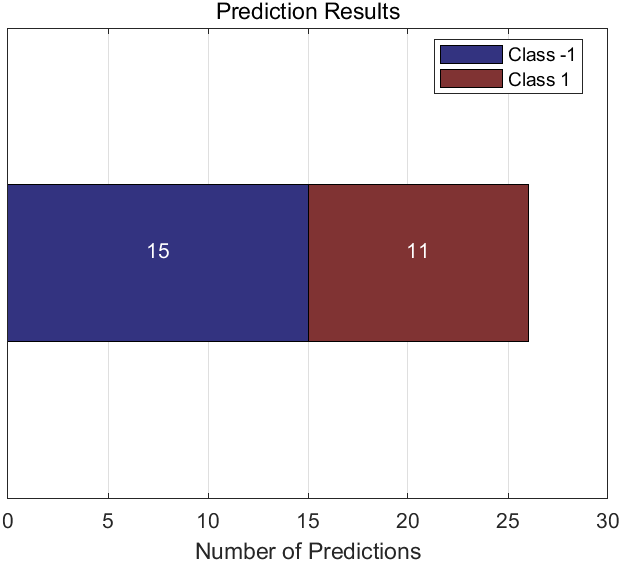
\includegraphics[width=0.95\linewidth]{bayes1.png} % Adjust the scale as needed
    \caption{Prediction results}
    \label{fig:prediction_results}
  \end{minipage}%
  \begin{minipage}{0.5\textwidth}
    \centering
    \resizebox{0.95\linewidth}{!}{% Resize table to fit within minipage if necessary
    \begin{tabular}{|c|c|c|c|c|c|}
      \hline
      \multicolumn{6}{|c|}{Means} \\ \hline
      Class '-1' & 1.0517 & 1.7996 & 0.8596 & 1.0642 & 1.0086 \\ \hline
      Class '1' & 0.0138 & -0.8876 & 0.0846 & -0.1548 & 0.0228 \\ \hline
      \multicolumn{6}{|c|}{Variances} \\ \hline
      Class '-1' & 1.0478 & 0.8390 & 1.0972 & 1.0378 & 1.0204 \\ \hline
      Class '1' & 1.1204 & 0.9384 & 0.8522 & 0.9465 & 1.1696 \\ \hline
    \end{tabular}
    }
    \caption{Mean and Variance Vectors for Two Categories}
    \label{tab:mean_variance}
  \end{minipage}
\end{figure}




\subsection{Gaussian Naïve Bayes Classifier}

In the realm of probabilistic classifiers, the Naive Bayes classifier stands out for its simplicity and effectiveness, especially in tasks involving high-dimensional data. There are primarily three variants of the Naive Bayes classifier, each tailored to a specific type of data distribution: the Gaussian Naive Bayes for continuous data, the Bernoulli Naive Bayes for binary data, and the Multinomial Naive Bayes for count or frequency data.

For this project, the data under consideration is continuous, as demonstrated by the first eight training samples shown in Table \ref{tab:training_samples}. The Gaussian Naive Bayes classifier is thus the appropriate choice for modeling this type of data. The Gaussian Naive Bayes assumes that the likelihood of the features is Gaussian distributed, which is a reasonable assumption when dealing with continuous data.

The class-conditional probability density function for a continuous feature  \( X \), under the assumption of a Gaussian distribution, is expressed as:

\[
p(x|\omega_j) = \frac{1}{\sqrt{2\pi\sigma_j}} \exp \left(-\frac{1}{2} \left(\frac{x - \mu_j}{\sigma_j}\right)^2\right)
\]

where \( \mu_j \) is the mean and \( \sigma_j \) is the variance of the feature for class \( \omega_j \).



% Table with the first eight training samples and their classes
\begin{table}[htbp]
\centering
\caption{First Eight Training Samples and Their Class Labels}
\begin{tabular}{ccccccc}
\hline
Feature 1 & Feature 2 & Feature 3 & Feature 4 & Feature 5  & Class Label \\
\hline
-1.3077 & -1.1742 & 0.1093 & -0.9395 & -3.0730  & 1 \\
-0.4336 & -0.1922 & 1.8140 & -0.0375 & 0.6263  & 1 \\
0.3426 & -0.2741 & 0.3120 & -1.8963 & -0.2867  & 1 \\
3.5784 & 1.5301 & 1.8045 & -2.1280 & -0.1973  & 1 \\
2.7694 & -0.2490 & -0.7231 & -1.1769 & 0.4056  & 1 \\
-1.3499 & -1.0642 & 0.5265 & -0.9905 & -1.4193 & 1 \\
3.0349 & 1.6035 & -0.2603 & -1.1730 & -0.7294 & 1 \\
0.7254 & 1.2347 & 0.6001 & -1.7254 & 1.1473 &  1 \\
\hline
\end{tabular}
\label{tab:training_samples}
\end{table}

Below we reproduce the corresponding code according to the principle. Prior probabilities represent the initial likelihood of each class in the dataset. They are calculated based on the frequency of each class in the training set without considering the feature values:

\begin{minted}{matlab}
% Calculating a priori probabilities
unique_labels = unique(label_train);
num_classes = numel(unique_labels);
priors = zeros(num_classes, 1);
for i = 1:num_classes
    priors(i) = sum(label_train == unique_labels(i)) / numel(label_train);
end
\end{minted}

Under the Gaussian Naïve Bayes variant, the feature distribution given the class label is assumed to be Gaussian. The mean and variance of each feature for each class are estimated using the training data. This assumption allows us to model the conditional probability of a feature given a class for continuous data:

\begin{minted}{matlab}
% Estimating conditional probability densities
means = zeros(num_classes, num_features);
variances = zeros(num_classes, num_features);
for i = 1:num_classes
    class_data = data_train(label_train == unique_labels(i), :);
    means(i, :) = mean(class_data, 1);
    variances(i, :) = var(class_data, 0, 1); % Using sample variance
end
\end{minted}

For classification, the posterior probability of each class given an observation is calculated using the Bayes' theorem. The class with the highest posterior probability is then chosen as the predicted class for that observation:

\begin{minted}{matlab}
% Categorized test data
predicted_labels1 = zeros(size(data_test, 1), 1);
for i = 1:size(data_test, 1)
    posteriors = zeros(num_classes, 1);
    for j = 1:num_classes
        likelihood = normpdf(data_test(i, :), means(j, :), sqrt(variances(j, :)));
        posteriors(j) = prod(likelihood) * priors(j);
    end
    [~, predicted_index] = max(posteriors);
    predicted_labels1(i) = unique_labels(predicted_index);
    disp(['Sample ' num2str(i) ', Predicted label: ' num2str(predicted_labels1(i))]);
end
\end{minted}

The application of the Naive Bayes classifier to our test dataset has yielded definitive predictions for the classification of instances into the respective categories. As illustrated in the histogram (Figure \ref{fig:naive_bayes_results}), the classifier assigned 15 instances to Class -1 and 11 instances to Class 1, demonstrating the effectiveness of the Naive Bayes approach in discriminative classification tasks. Remarkably, these results are consistent with those obtained using the Bayesian decision classifier, reaffirming the reliability and robustness of Bayesian techniques in statistical inference and decision-making under uncertainty.

\begin{figure}[htbp]
\centering
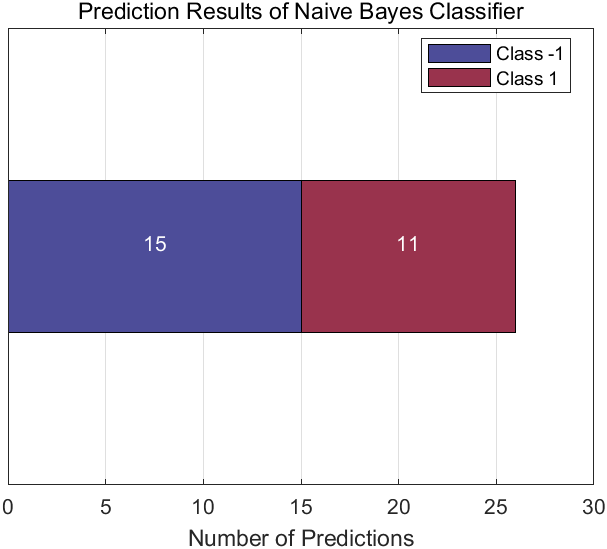
\includegraphics[width=0.8\linewidth]{Naive Bayes.png}
\caption{Prediction results of the Naive Bayes classifier showing the number of test samples classified into each class.}
\label{fig:naive_bayes_results}
\end{figure}



\subsection{Linear Discriminant Analysis classifier}
Linear Discriminant Analysis (LDA) is a statistical approach used for the classification and dimensionality reduction of data. LDA seeks to project the data onto a lower-dimensional space with good class-separability in order to avoid overfitting ("curse of dimensionality") and also reduce computational costs.

The linear discriminant function, which is used to classify samples, can be expressed as:
\[
g(\mathbf{x}) = \mathbf{w}^T\mathbf{x} + w_0
\]
Where \( \mathbf{w} \) is the weight vector and \( w_0 \) is the bias or threshold weight.

The maximization criterion for LDA, \( J(\mathbf{w}) \), is defined as the ratio of the determinant of the between-class scatter matrix \( S_B \) to the within-class scatter matrix \( S_W \), which can be expressed as:
\[
J(\mathbf{w}) = \frac{\mathbf{w}^T S_B \mathbf{w}}{\mathbf{w}^T S_W \mathbf{w}}
\]

The methodology of LDA involves the following steps:

\begin{enumerate}
    \item Compute the mean vectors \( m_1 \) and \( m_2 \) for the two classes.
    \item Calculate the within-class scatter matrix \( S_W \).
    \item Derive the weight vector \( \mathbf{w} \) which maximizes the criterion \( J(\mathbf{w}) \).
    \item Construct the discriminant function \( g(\mathbf{x}) \) for classification.
\end{enumerate}

The goal is to find the optimal weight vector \( \mathbf{w} \) that maximizes the between-class scatter while minimizing the within-class scatter, effectively separating the classes in the projected space.

The initialization phase involves setting up the basic parameters required for LDA, including the number of features, the unique labels in the target variable, and the total number of classes.

\begin{minted}{matlab}
% Initialization
num_features = size(data_train, 2);
unique_labels = unique(label_train);
num_classes = numel(unique_labels);
\end{minted}

Following initialization, the next step is to calculate the mean vectors for each class. These mean vectors are critical as they represent the central point of each class in the feature space.

\begin{minted}{matlab}
% Compute class means
means = zeros(num_classes, num_features);
for i = 1:num_classes
    means(i, :) = mean(data_train(label_train == unique_labels(i), :), 1);
end
\end{minted}

The overall mean of the data is also computed, which will be used later in calculating the between-class scatter matrix.

\begin{minted}{matlab}
% Compute overall mean
overall_mean = mean(data_train, 1);
\end{minted}

With the class and overall means calculated, we proceed to determine the within-class and between-class scatter matrices. These matrices measure the scatter (or spread) of the class samples around the class mean and the overall mean, respectively.

\begin{minted}{matlab}
% Compute within-class and between-class scatter matrices
Sw = zeros(num_features, num_features); 
Sb = zeros(num_features, num_features); 
for i = 1:num_classes
    class_data = data_train(label_train == unique_labels(i), :);
    class_mean = means(i, :);
    Sw = Sw + (class_data - class_mean).' * (class_data - class_mean);
    Sb = Sb + size(class_data, 1) * (class_mean - overall_mean).' * 
    (class_mean - overall_mean);
end
\end{minted}

To ensure that the within-class scatter matrix is non-singular, a small regularization term is added. This is crucial for computing the eigenvalues and eigenvectors in the subsequent steps.

\begin{minted}{matlab}
% Add regularization to prevent singularity of Sw
Sw = Sw + eye(size(Sw)) * 1e-4;  % Small regularization term
\end{minted}

The optimal projection direction that maximizes the separation between classes is found by solving the generalized eigenvalue problem. The eigenvectors corresponding to the largest eigenvalues will form the projection matrix. \textbf{In this example, the largest eigenvalue in the previous dimension is taken and the corresponding vector, i.e., the decision boundary, is a point.}

\begin{minted}{matlab}
% Compute optimal projection direction
[V, D] = eig(Sb, Sw);
[~, order] = sort(diag(D), 'descend');
%Select the first {number of categories - 1} components
W = V(:, order(1:num_classes-1)); 
\end{minted}

The final steps involve projecting the training data onto the new subspace and using the projected means to classify the test data.

\begin{minted}{matlab}
% Project training data
projected_data = data_train * W;

% Compute projected means
projected_means = means * W;

% Classify test data
predicted_labels = zeros(size(data_test, 1), 1);
for i = 1:size(data_test, 1)
    % Project test sample
    projected_sample = data_test(i, :) * W;
    % Compute distance to each class mean
    distances = pdist2(projected_sample, projected_means);
    % Choose the nearest class
    [~, min_index] = min(distances);
    predicted_labels(i) = unique_labels(min_index);
    disp(['Sample ' num2str(i) ', Predicted label: ' num2str(predicted_labels(i))]);
end
\end{minted}

The final results are shown in Figure \ref{fig:lda_results} and Figure \ref{fig:lda_projection}. Figure \ref{fig:lda_results} represents the final classification results of LDA with the corresponding number of each category, which can be seen to be identical to the results of the first two classifiers! Finally, we draw the test dataset with points being projected onto the eigenvector corresponding to the first principal component eigenvalue, as shown in Figure \ref{fig:lda_projection}. It can be seen that the points of the test data samples have the largest scatter of the projections in that direction and can be decisively classified.

\begin{figure}[htbp]
\centering
\begin{minipage}[b]{0.48\linewidth}
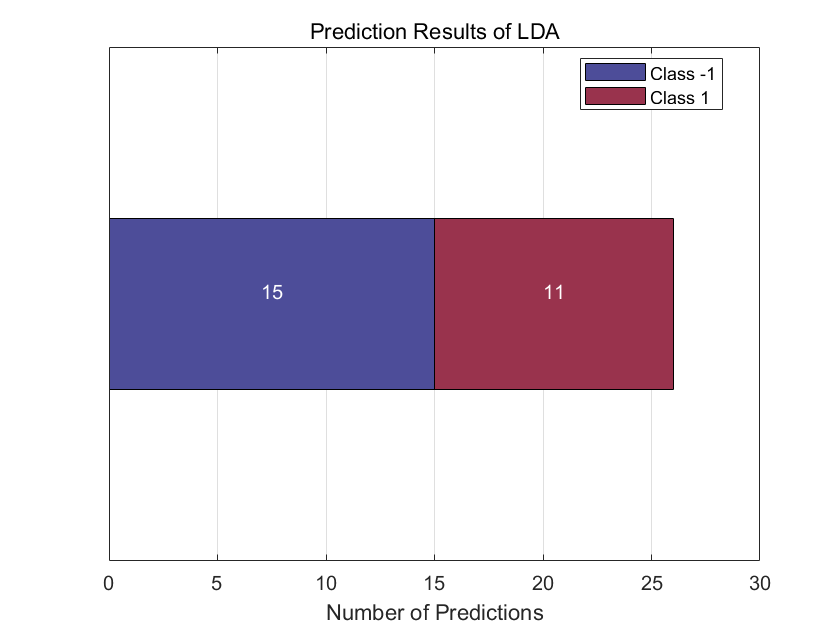
\includegraphics[width=\linewidth]{LDA2.png}
\caption{Prediction results of LDA.}
\label{fig:lda_results}
\end{minipage}
\hfill
\begin{minipage}[b]{0.48\linewidth}
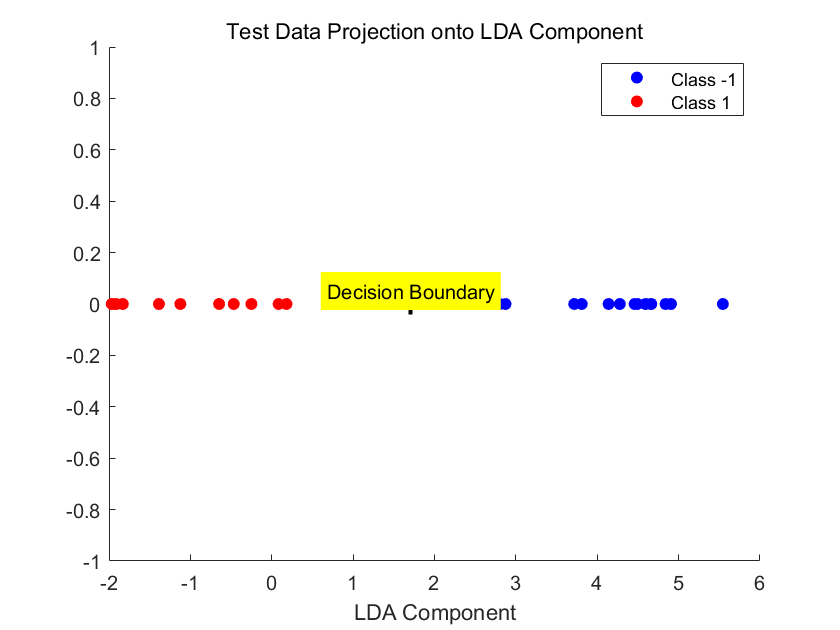
\includegraphics[width=\linewidth]{untitled111.png}
\caption{Test data projection onto LDA component.}
\label{fig:lda_projection}
\end{minipage}
\end{figure}



\subsection{Analysis of Results}

As shown in Table \ref{tab:classification_across_classifiers}, it is intriguing to observe that the Bayes decision rule, Gaussian Naïve Bayes, and Linear Discriminant Analysis (LDA) classifiers all yield identical classification outcomes for the test dataset. This consistency across different classification approaches suggests several implications about the dataset and the underlying assumptions of these models.

Firstly, the similar performance of the Bayes decision rule and Gaussian Naïve Bayes classifier could be attributed to the distribution of the data. Naïve Bayes classifiers assume that the features are independent given the class label, and they perform well if this assumption is not severely violated. If the dataset's features are indeed approximately conditionally independent or the dependencies do not significantly impact the posterior probabilities, both classifiers would render similar predictions.

Secondly, the LDA's identical classification results indicate that the data is likely to be linearly separable. LDA assumes that different classes generate data based on different Gaussian distributions with the same covariance matrix. If the test data follows a Gaussian distribution with equal covariance matrices for both classes, then LDA would perform similarly to the Bayes classifiers, which also incorporate Gaussian likelihoods.

The consistent results might also be a sign that the dataset is not complex and can be easily separated with a linear decision boundary, making more sophisticated models unnecessary. It is also possible that the dataset size is not large enough or not varied enough to differentiate the performance of these classifiers, or the features chosen are highly discriminative, leading to a scenario where all classifiers reach their performance plateau.

In contrast, datasets with more complex, non-linear boundaries or those that violate the independence assumption would likely result in diverging performances from these classifiers. Therefore, while the consistency in classifier performance simplifies the model selection process in this scenario, it is also a prompt to scrutinize the data characteristics more closely and consider whether the dataset and feature set are representative and challenging enough for the problem at hand.

In conclusion, the identical performance of the three different classifiers points to a dataset that fits well within the assumptions of Gaussian distributions and linear separability. It is recommended to explore the dataset further with more complex models and additional features, especially if the dataset will be used in more challenging real-world conditions where these assumptions may not hold true.

\begin{landscape}
\begin{table}[htbp]
\centering
\caption{Summary of Classification Results Across Classifiers}
\label{tab:classification_across_classifiers}
\resizebox{\columnwidth}{!}{% Resize table to fit within column width
\begin{tabular}{cccc|c}
\toprule
\textbf{Sample Number} & \textbf{Bayes decision rule} & \textbf{Gaussian Naïve Bayes} & \textbf{Linear Discriminant Analysis} & \textbf{Count} \\
\midrule
1 & -1 & -1 & -1 \\
2 & -1 & -1 & -1 \\
3 & -1 & -1 & -1 \\
4 & -1 & -1 & -1 \\
5 & -1 & -1 & -1 \\
6 & -1 & -1 & -1 \\
7 & -1 & -1 & -1 \\
8 & -1 & -1 & -1 \\
9 & -1 & -1 & -1 \\
10 & -1 & -1 & -1 \\
11 & -1 & -1 & -1 \\
12 & -1 & -1 & -1 \\
13 & -1 & -1 & -1 \\
14 & -1 & -1 & -1 & 15 \\
\midrule
15 &  1 & 1 & 1 & \\
16 & 1 & 1 & 1 \\
17 & 1 & 1 & 1 \\
18 & 1 & 1 & 1 \\
19 & 1 & 1 & 1 \\
20 & 1 & 1 & 1 \\
21 & 1 & 1 & 1 \\
22 & 1 & 1 & 1 \\
23 & 1 & 1 & 1 \\
24 & 1 & 1 & 1 \\
25 & 1 & 1 & 1 \\
26 & 1 & 1 & 1 & 11 \\
\bottomrule
\end{tabular}
}
\end{table}
\end{landscape}

\section{Assignment 2}
\subsection{Raw Data Analysis}
Still, we started with a preliminary data analysis to understand the distribution of the dataset. The "TrainingData.xlsx" sample was analyzed, focusing on category class, number of data points, dimensionality, and number of test samples. The histogram in Figure \ref{fig:class_histogram1} shows the distribution of categories in the training set, and it can be seen that there are three categories, and the number of sample points for each category is labeled; Figure \ref{fig:pca_scatter1} shows the scatter distribution of the data. Since the dimension of the sample points is 4, it is not convenient to visualize their distribution, so we first use PCA to reduce them to 2 dimensions in order to show their distribution on the first two main eigenvectors, and Figure \ref{fig:pca_scatter1} shows the scatterplot after the PCA reduction, in order to show the discrete characteristics of the data.

\begin{figure}[htbp]
\centering
\begin{minipage}[b]{0.48\linewidth}
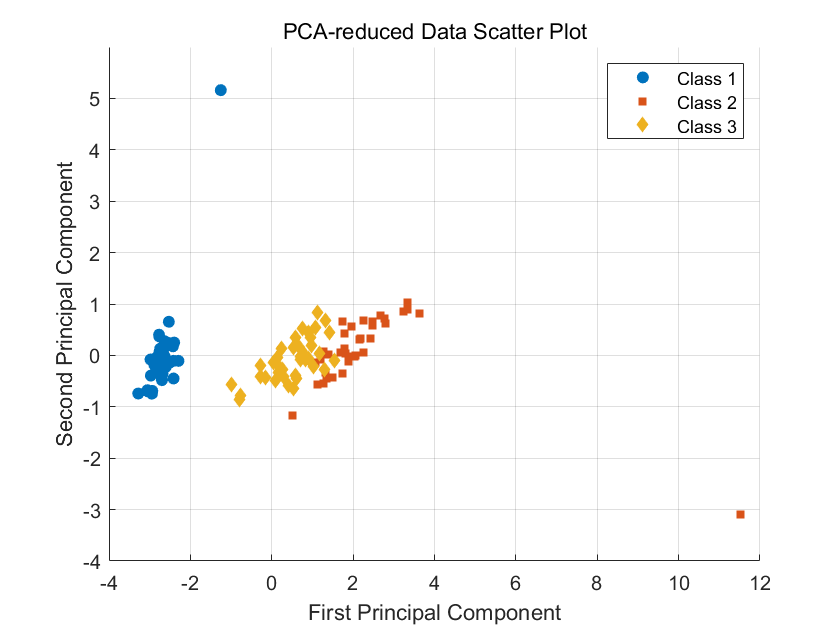
\includegraphics[width=\linewidth]{1.png}
\caption{PCA-reduced Data Scatter Plot.}
\label{fig:pca_scatter1}
\end{minipage}
\hfill
\begin{minipage}[b]{0.48\linewidth}
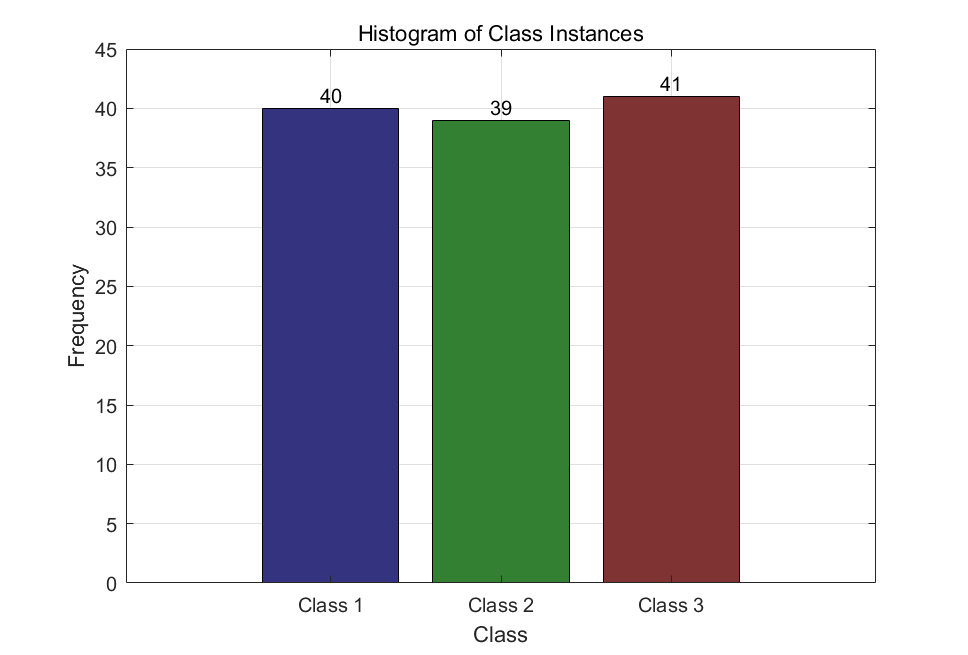
\includegraphics[width=\linewidth]{2.png}
\caption{Histogram of Class Instances of "TrainingData.xlsx".}
\label{fig:class_histogram1}
\end{minipage}
\end{figure}

The PCA scatter plot in Figure \ref{fig:pca_scatter1} reveals the presence of potential outliers, particularly noticeable for Class 1$\&$2 where a few data points deviate significantly from the main cluster. These outliers could be a result of measurement errors, data entry mistakes, or genuine rare occurrences and warrant further investigation to determine whether they should be retained or treated before model training.

Conversely, the histogram in Figure \ref{fig:class_histogram1} indicates a relatively uniform distribution of data points across the three classes, which is desirable in a training set. Such a balance suggests that the classifier will be less likely to develop a bias towards any particular class due to the sample size and can be trained to recognize each class with equal emphasis. The uniformity in class distribution lays a solid foundation for training robust classification models.

Let's deal with missing values and outliers in the data, starting with the code for missing value discrimination:
\begin{minted}{matlab}
% Checking for missing values
if any(any(ismissing(trainingData)))
    % Handling Missing Values
    trainingData = rmmissing(trainingData);
end
\end{minted}

There are no missing values in the data and the next step is to check for outliers. Outliers in the dataset were detected using a standard deviation threshold method. For each feature, a z-score was computed and data points that had a feature with a z-score exceeding the threshold of 3 in absolute value were flagged as potential outliers. As shown in the Table \ref{tab:outliers}, two outliers were detected, as we observed from Figure \ref{fig:pca_scatter1} in agreement with the results! The MATLAB code used for the detection of outliers is presented below:

\begin{minted}{matlab}
% Compute z-scores for each feature
zScores = (trainingData{:,1:end-1} - mean(trainingData{:,1:end-1})) ./ 
          std(trainingData{:,1:end-1});
% Define the threshold for outliers
threshold = 3;
% Find indices of outliers
outlierIndices = any(abs(zScores) > threshold, 2);
% Select the outliers
outliers = trainingData(outlierIndices, :);
% Display the outliers
disp('Detected outliers:');
disp(outliers);
\end{minted}


\begin{table}[ht]
\centering
\caption{Detected outliers with their corresponding true labels (Var5).}
\label{tab:outliers}
\begin{tabular}{ccccc}
\toprule
Var1 & Var2 & Var3 & Var4 & Class\_label \\
\midrule
6.3 & 3.3 & 16 & 2.5 & 2 \\
5.7 & 4.4 & 1.5 & 0.4 & 1 \\
\bottomrule
\end{tabular}
\end{table}

To handle outliers, we use the mean of each feature within the sample class in place of outliers.

\begin{minted}{matlab}
% Replacing outliers with averages
for i = 1:size(outlierIndices,2)
    feature_outliers = outlierIndices(:,i);
    trainingData{feature_outliers,i} = means(i);
end
\end{minted}

\subsection{Binary classification tree}
After replacing the outliers, we again output the scatterplot of the data that was downscaled to 2 dimensions using PCA, as shown in Figure \ref{fig:remove}, which shows that the data is very compactly distributed and no outliers appear.

\begin{figure}[htbp]
\centering
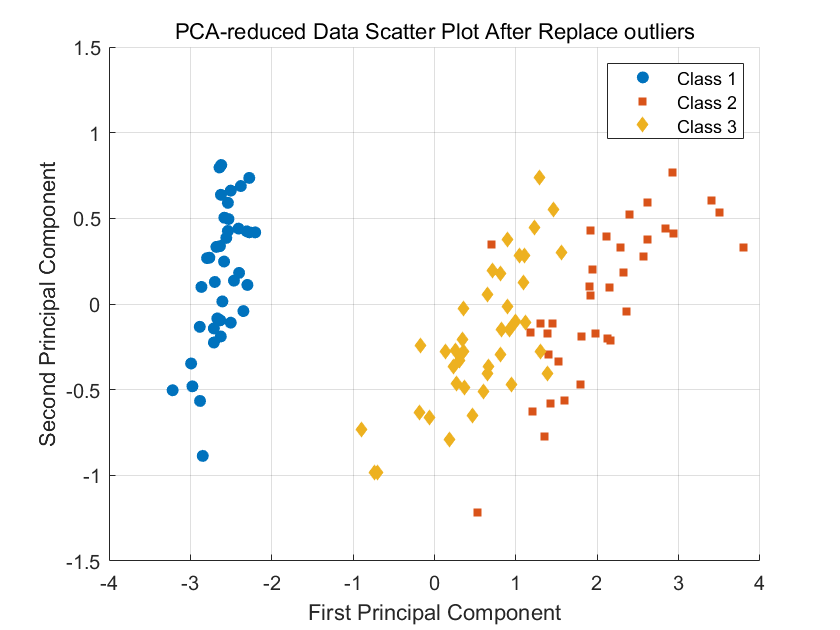
\includegraphics[width=0.8\linewidth]{33.png}
\caption{PCA-reduced Data Scatter Plot After Replace outliers.}
\label{fig:remove}
\end{figure}

Before training the decision tree, it is essential to determine the most informative features and their respective splitting points that will form the nodes of the tree. The Gini impurity measure is used for this purpose, as it quantifies the impurity of a potential split. Figures \ref{fig:gini_impurity_4} show the Gini impurity plotted against different splitting points for each feature. These plots were crucial in identifying the thresholds that minimize impurity, and thus, determine where the data is split at each node of the decision tree.

\begin{figure}[htbp]
\centering
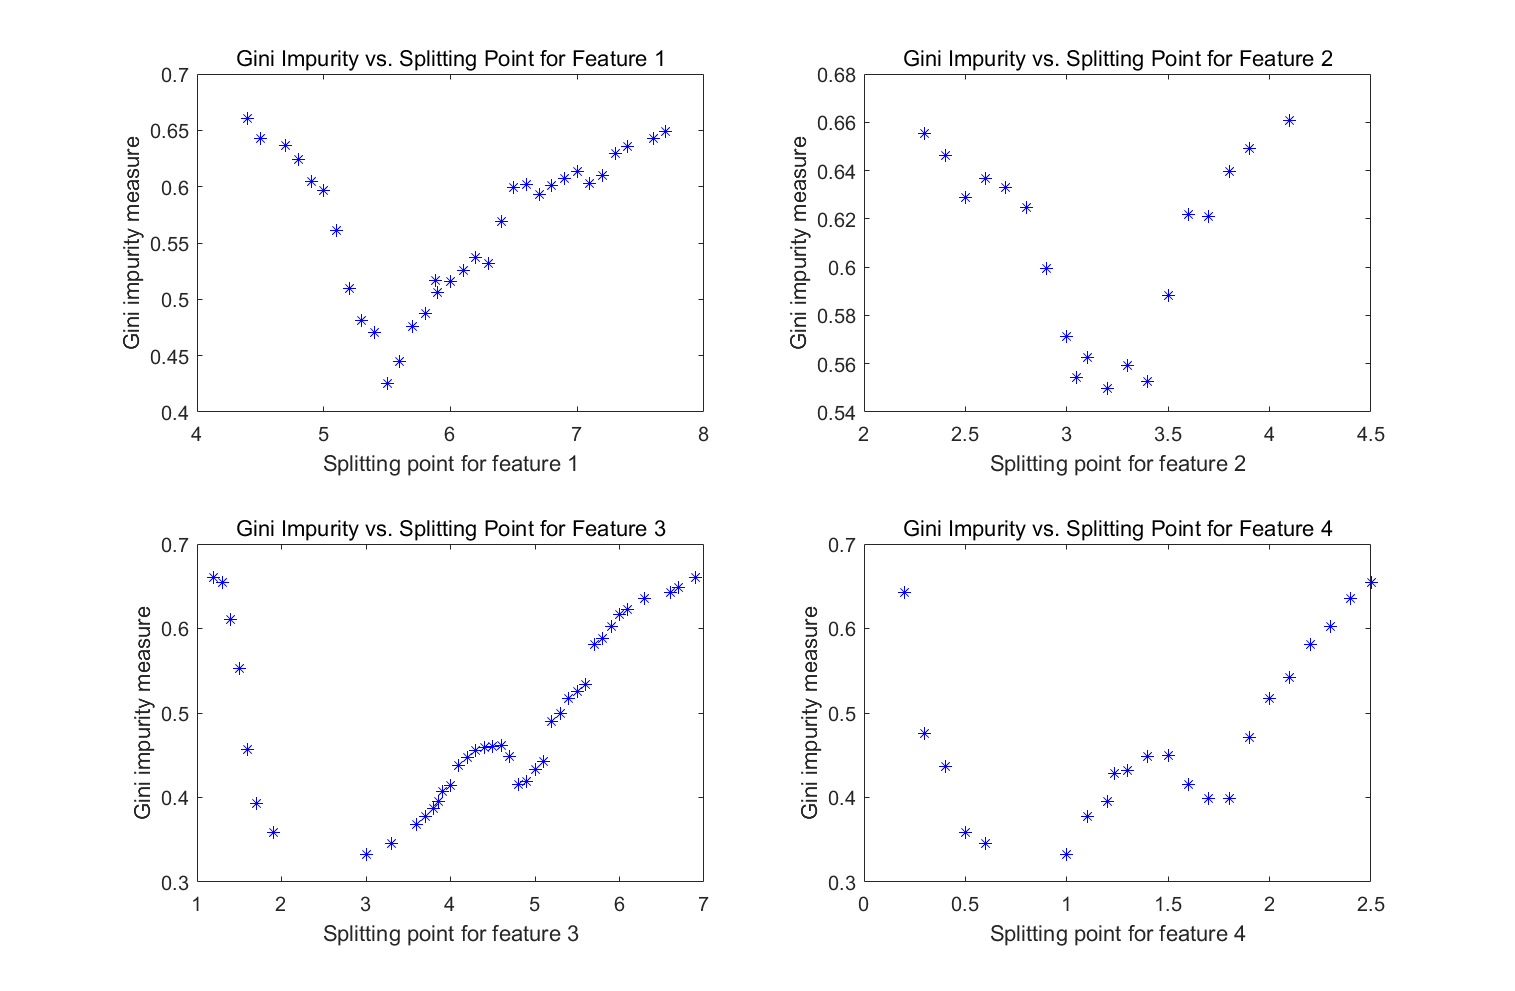
\includegraphics[width=0.8\linewidth]{222.png}
\caption{Gini Impurity vs. Splitting Point.}
\label{fig:gini_impurity_4}
\end{figure}

Following the selection of the best splitting points based on the Gini impurity, the decision tree was trained. The resulting structure of the tree is depicted in Figure \ref{fig:decision_tree}, showing how the data is split at each node. The nodes represent the feature and threshold that lead to the best separation at that point in the tree, while the leaves represent the final classification outcome.

\begin{figure}[htbp]
\centering
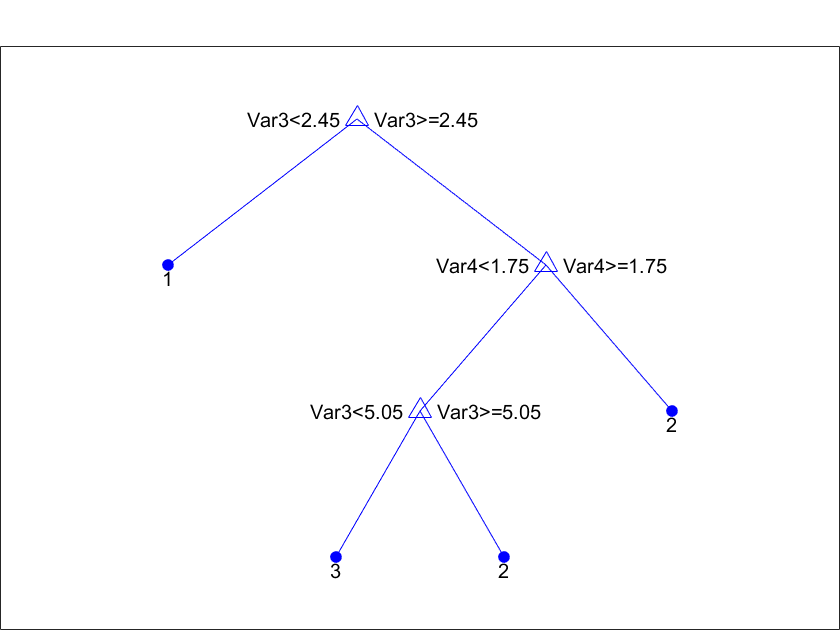
\includegraphics[width=0.8\linewidth]{1111.png}
\caption{Visualization of the trained decision tree.}
\label{fig:decision_tree}
\end{figure}


The process of training a binary classification tree on a preprocessed dataset is shown in detail below. The first step involves separating the features from the labels, which are then used to train the model through a recursive function. The code below demonstrates the training procedure, which includes the construction of the decision tree through recursive partitioning of the dataset based on the best feature and threshold found at each node. It also outlines the prediction process where a new record is classified by traversing the decision tree.

\begin{minted}{matlab}
% Train binary classification tree
% Separate features and labels
features = trainingData(:, 1:end-1);
labels = trainingData(:, end);
% Train the model
root = trainDecisionTree(features, labels);

% Perform predictions
% Ensure testData is a numeric array
if istable(testData)
    testData = table2array(testData);
end

% Initialize an array to store predicted labels
predictions = zeros(size(testData, 1), 1);

% Predict for each test sample
for i = 1:size(testData, 1)
    predictions(i) = predictDecisionTree(root, testData(i, :));
end

disp('Predicted labels:');
disp(predictions);

\end{minted}



The function \texttt{trainDecisionTree} is designed to recursively build the decision tree from the training data. It evaluates the conditions for stopping the recursion and creating a leaf node. If no stopping condition is met, it chooses the best feature and threshold to split the data, then recursively creates the left and right subtrees.

\begin{minted}{matlab}
function node = trainDecisionTree(data, labels)
    % Convert input data to numeric arrays if they are tables
    if istable(data)
        data = table2array(data);
    end
    if istable(labels)
        labels = table2array(labels);
    end

    % Return a leaf node if all labels are the same
    if numel(unique(labels)) == 1
        node.isLeaf = true;
        node.label = labels(1);
        return;
    end

    % Return a leaf node if all data points have the same feature values
    if all(var(data, 0, 1) == 0)
        node.isLeaf = true;
        % Choose the most common label as the leaf label
        node.label = mode(labels);
        return;
    end

    % Initialize the node
    node.isLeaf = false;
    node.predicate = [];
    node.left = [];
    node.right = [];
    node.label = [];

    % Select the best splitting feature
    [bestFeature, bestThreshold] = chooseBestFeatureToSplit(data, labels);

    % Check for a valid split feature
    if bestFeature <= 0
        node.isLeaf = true;
        node.label = mode(labels);
        return;
    end

    node.predicate = @(record) record(bestFeature) < bestThreshold;

    % Split the dataset
    leftIndices = data(:, bestFeature) < bestThreshold;
    rightIndices = ~leftIndices;

    % Recursively build left and right subtrees
    if sum(leftIndices) == 0 || sum(rightIndices) == 0
        node.isLeaf = true;
        node.label = mode(labels);
        return;
    else
        node.left = trainDecisionTree(data(leftIndices, :), labels(leftIndices));
        node.right = trainDecisionTree(data(rightIndices, :), labels(rightIndices));
    end
end
\end{minted}


The function \texttt{chooseBestFeatureToSplit} finds the feature and threshold that lead to the best split based on the minimization of error. It iterates over all features and their possible thresholds to identify the split that yields the smallest error.

\begin{minted}{matlab}
function [bestFeature, bestThreshold] = chooseBestFeatureToSplit(data, labels)
    % A simplified feature selection function based on minimum error
    numFeatures = size(data, 2);
    bestError = inf;
    bestFeature = 0;
    bestThreshold = 0;

    % Ensure labels are a numeric array
    if istable(labels)
        labels = table2array(labels);
    end

    for i = 1:numFeatures
        % Ensure the feature column is a numeric array
        featureValues = data(:, i);
        thresholds = unique(featureValues);
        for thresholdIndex = 1:length(thresholds)
            threshold = thresholds(thresholdIndex);
            predictions = featureValues < threshold;
            error = sum(predictions ~= labels);
            if error < bestError
                bestError = error;
                bestFeature = i;
                bestThreshold = threshold;
            end
        end
    end
    if bestFeature == 0
        fprintf('No valid feature was found to split the data.\n');
    end
end
\end{minted}

Once the decision tree is constructed, the \texttt{predictDecisionTree} function is used to classify new records. It traverses the tree according to the predicates at each node until it reaches a leaf node, where it returns the predicted label.

\begin{minted}{matlab}
function label = predictDecisionTree(node, record)
    % Return the predicted label if a leaf node is reached
    if node.isLeaf
        label = node.label;
        return;
    end
    % Choose left or right branch based on the predicate
    if node.predicate(record)
        label = predictDecisionTree(node.left, record);
    else
        label = predictDecisionTree(node.right, record);
    end
end
\end{minted}
Eventually, the results of latex classification are shown in the \ref{tab:features_and_predictions}.

\begin{table}[ht]
\centering
\caption{Features and Prediction Results for Samples}
\label{tab:features_and_predictions}
\begin{tabular}{cccccc}
\toprule
Sample Index & Feature 1 & Feature 2 & Feature 3 & Feature 4 & Predicted Class \\
\midrule
1 & 4.8 & 3.1 & 1.6 & 0.2 & 1\\
2 & 5.1 & 3.5 & 1.4 & 0.3 & 1 \\
3 & 4.8 & 3 & 1.4 & 0.1 & 1\\
4 & 5.7 & 3.8 & 1.7 & 0.3 & 1\\
5 & 5.5 & 4.2 & 1.4 & 0.2 & 1\\
6 & 5 & 3.4 & 1.5 & 0.2 & 1\\
7 & 4.6 & 3.1 & 1.5 & 0.2 & 1\\
8 & 5.8 & 4 & 1.2 & 0.2 & 1\\
9 & 5 & 3.6 & 1.4 & 0.2 & 1\\
10 & 4.6 & 3.4 & 1.4 & 0.3 & 1\\
11 & 6 & 2.2 & 5 & 1.5 & 3\\
12 & 6.5 & 3.2 & 5.1 & 2 & 2\\
13 & 7.7 & 3 & 6.1 & 2.3 & 2\\
14 & 6.9 & 3.2 & 5.7 & 2.3 & 2\\
15 & 7.9 & 3.8 & 6.4 & 2 & 2\\
16 & 6.5 & 3 & 5.2 & 2 & 2\\
17 & 6.2 & 2.8 & 4.8 & 1.8 & 2\\
18 & 6.7 & 2.5 & 5.8 & 1.8 & 2\\
19 & 6.2 & 3.4 & 5.4 & 2.3 & 2\\
20 & 6.5 & 3 & 5.5 & 1.8 & 2\\
21 & 6.8 & 3 & 5.5 & 2.1 & 2\\
22 & 5.8 & 2.7 & 4.1 & 1 & 3\\
23 & 6.8 & 2.8 & 4.8 & 1.4 & 3\\
24 & 6.7 & 3.1 & 4.4 & 1.4 & 3\\
25 & 5.2 & 2.7 & 3.9 & 1.4 & 3\\
26 & 5.7 & 2.6 & 3.5 & 1 & 3\\
27 & 5.6 & 2.5 & 3.9 & 1.1 & 3\\
28 & 5.5 & 2.5 & 4 & 1.3 & 3\\
29 & 5 & 2 & 3.5 & 1 & 3\\
30 & 6.4 & 3.2 & 4.5 & 1.5 & 3\\
\bottomrule
\end{tabular}
\end{table}

The Gini impurity graphs, shown in Figures \ref{fig:gini_feature4}, provided valuable insights into the selection of the splitting points for the decision tree. These plots were crucial for identifying the thresholds that minimize impurity at each split, enabling the decision tree to effectively partition the data into homogenous subsets.

Figure \ref{fig:gini_feature4} suggests that Feature 1 has a potential split point around 5.6, where the Gini impurity reaches a local minimum, indicating an optimal separation of the classes. However, this feature was not selected as the root split in the final tree structure, which suggests that while it may offer some class separation, other features provide a more significant reduction in impurity.

On the other hand, Feature 3 exhibits a clear trend in Gini impurity (see Figure \ref{fig:gini_feature4}), and a distinct threshold at 5.05 was chosen for a split. This choice is corroborated by the decision tree visualization in Figure \ref{fig:decision_tree}, where Var3 indeed appears as a prominent node, bifurcating the data into two distinct classes.

Figure \ref{fig:decision_tree} provides a visual representation of the trained decision tree. The topmost split based on Var3 divides the samples into two groups, with one group predominantly consisting of a single class, as evidenced by the leaf node labeled '1'. Further splits based on Var4 fine-tune the separation, especially for those samples that were not clearly classified at the first node.

This decision tree structure highlights the model's ability to discern patterns in the feature space that correlate with the different classes. The resulting classification boundaries capture the distinctions learned from the training data, as seen in the purity of the leaf nodes.

Through this analysis, we observe that the decision tree prioritizes splits on features that lead to the largest gain in purity. The depth of the tree and the sequence of features chosen for the splits reflect the model's strategy to optimize class separation.


\end{document}